% Options for packages loaded elsewhere
\PassOptionsToPackage{unicode}{hyperref}
\PassOptionsToPackage{hyphens}{url}
\PassOptionsToPackage{dvipsnames,svgnames,x11names}{xcolor}
%
\documentclass[
  letterpaper,
  DIV=11,
  numbers=noendperiod]{scrartcl}

\usepackage{amsmath,amssymb}
\usepackage{iftex}
\ifPDFTeX
  \usepackage[T1]{fontenc}
  \usepackage[utf8]{inputenc}
  \usepackage{textcomp} % provide euro and other symbols
\else % if luatex or xetex
  \usepackage{unicode-math}
  \defaultfontfeatures{Scale=MatchLowercase}
  \defaultfontfeatures[\rmfamily]{Ligatures=TeX,Scale=1}
\fi
\usepackage{lmodern}
\ifPDFTeX\else  
    % xetex/luatex font selection
\fi
% Use upquote if available, for straight quotes in verbatim environments
\IfFileExists{upquote.sty}{\usepackage{upquote}}{}
\IfFileExists{microtype.sty}{% use microtype if available
  \usepackage[]{microtype}
  \UseMicrotypeSet[protrusion]{basicmath} % disable protrusion for tt fonts
}{}
\makeatletter
\@ifundefined{KOMAClassName}{% if non-KOMA class
  \IfFileExists{parskip.sty}{%
    \usepackage{parskip}
  }{% else
    \setlength{\parindent}{0pt}
    \setlength{\parskip}{6pt plus 2pt minus 1pt}}
}{% if KOMA class
  \KOMAoptions{parskip=half}}
\makeatother
\usepackage{xcolor}
\setlength{\emergencystretch}{3em} % prevent overfull lines
\setcounter{secnumdepth}{-\maxdimen} % remove section numbering
% Make \paragraph and \subparagraph free-standing
\makeatletter
\ifx\paragraph\undefined\else
  \let\oldparagraph\paragraph
  \renewcommand{\paragraph}{
    \@ifstar
      \xxxParagraphStar
      \xxxParagraphNoStar
  }
  \newcommand{\xxxParagraphStar}[1]{\oldparagraph*{#1}\mbox{}}
  \newcommand{\xxxParagraphNoStar}[1]{\oldparagraph{#1}\mbox{}}
\fi
\ifx\subparagraph\undefined\else
  \let\oldsubparagraph\subparagraph
  \renewcommand{\subparagraph}{
    \@ifstar
      \xxxSubParagraphStar
      \xxxSubParagraphNoStar
  }
  \newcommand{\xxxSubParagraphStar}[1]{\oldsubparagraph*{#1}\mbox{}}
  \newcommand{\xxxSubParagraphNoStar}[1]{\oldsubparagraph{#1}\mbox{}}
\fi
\makeatother


\providecommand{\tightlist}{%
  \setlength{\itemsep}{0pt}\setlength{\parskip}{0pt}}\usepackage{longtable,booktabs,array}
\usepackage{calc} % for calculating minipage widths
% Correct order of tables after \paragraph or \subparagraph
\usepackage{etoolbox}
\makeatletter
\patchcmd\longtable{\par}{\if@noskipsec\mbox{}\fi\par}{}{}
\makeatother
% Allow footnotes in longtable head/foot
\IfFileExists{footnotehyper.sty}{\usepackage{footnotehyper}}{\usepackage{footnote}}
\makesavenoteenv{longtable}
\usepackage{graphicx}
\makeatletter
\def\maxwidth{\ifdim\Gin@nat@width>\linewidth\linewidth\else\Gin@nat@width\fi}
\def\maxheight{\ifdim\Gin@nat@height>\textheight\textheight\else\Gin@nat@height\fi}
\makeatother
% Scale images if necessary, so that they will not overflow the page
% margins by default, and it is still possible to overwrite the defaults
% using explicit options in \includegraphics[width, height, ...]{}
\setkeys{Gin}{width=\maxwidth,height=\maxheight,keepaspectratio}
% Set default figure placement to htbp
\makeatletter
\def\fps@figure{htbp}
\makeatother

\KOMAoption{captions}{tableheading}
\makeatletter
\@ifpackageloaded{tcolorbox}{}{\usepackage[skins,breakable]{tcolorbox}}
\@ifpackageloaded{fontawesome5}{}{\usepackage{fontawesome5}}
\definecolor{quarto-callout-color}{HTML}{909090}
\definecolor{quarto-callout-note-color}{HTML}{0758E5}
\definecolor{quarto-callout-important-color}{HTML}{CC1914}
\definecolor{quarto-callout-warning-color}{HTML}{EB9113}
\definecolor{quarto-callout-tip-color}{HTML}{00A047}
\definecolor{quarto-callout-caution-color}{HTML}{FC5300}
\definecolor{quarto-callout-color-frame}{HTML}{acacac}
\definecolor{quarto-callout-note-color-frame}{HTML}{4582ec}
\definecolor{quarto-callout-important-color-frame}{HTML}{d9534f}
\definecolor{quarto-callout-warning-color-frame}{HTML}{f0ad4e}
\definecolor{quarto-callout-tip-color-frame}{HTML}{02b875}
\definecolor{quarto-callout-caution-color-frame}{HTML}{fd7e14}
\makeatother
\makeatletter
\@ifpackageloaded{caption}{}{\usepackage{caption}}
\AtBeginDocument{%
\ifdefined\contentsname
  \renewcommand*\contentsname{Table of contents}
\else
  \newcommand\contentsname{Table of contents}
\fi
\ifdefined\listfigurename
  \renewcommand*\listfigurename{List of Figures}
\else
  \newcommand\listfigurename{List of Figures}
\fi
\ifdefined\listtablename
  \renewcommand*\listtablename{List of Tables}
\else
  \newcommand\listtablename{List of Tables}
\fi
\ifdefined\figurename
  \renewcommand*\figurename{Figure}
\else
  \newcommand\figurename{Figure}
\fi
\ifdefined\tablename
  \renewcommand*\tablename{Table}
\else
  \newcommand\tablename{Table}
\fi
}
\@ifpackageloaded{float}{}{\usepackage{float}}
\floatstyle{ruled}
\@ifundefined{c@chapter}{\newfloat{codelisting}{h}{lop}}{\newfloat{codelisting}{h}{lop}[chapter]}
\floatname{codelisting}{Listing}
\newcommand*\listoflistings{\listof{codelisting}{List of Listings}}
\usepackage{amsthm}
\theoremstyle{definition}
\newtheorem{exercise}{Exercise}[section]
\theoremstyle{remark}
\AtBeginDocument{\renewcommand*{\proofname}{Proof}}
\newtheorem*{remark}{Remark}
\newtheorem*{solution}{Solution}
\newtheorem{refremark}{Remark}[section]
\newtheorem{refsolution}{Solution}[section]
\makeatother
\makeatletter
\makeatother
\makeatletter
\@ifpackageloaded{caption}{}{\usepackage{caption}}
\@ifpackageloaded{subcaption}{}{\usepackage{subcaption}}
\makeatother

\ifLuaTeX
  \usepackage{selnolig}  % disable illegal ligatures
\fi
\usepackage{bookmark}

\IfFileExists{xurl.sty}{\usepackage{xurl}}{} % add URL line breaks if available
\urlstyle{same} % disable monospaced font for URLs
\hypersetup{
  colorlinks=true,
  linkcolor={blue},
  filecolor={Maroon},
  citecolor={Blue},
  urlcolor={Blue},
  pdfcreator={LaTeX via pandoc}}


\author{}
\date{}

\begin{document}


\section{Dichtheidseffecten}\label{sec-dichtheid}

In het vorige onderdeel heb je geleerd dat een populatie in evenwicht is
als hun snelheid van verandering gelijk is aan 0. Zodoende bereikte de
populatie die eerst exponentiëel groeide, een evenwicht bij een bepaald
draagvermogen: de \textbf{carrying capacity}. In dit onderdeel gaan we
explicieter zijn over \emph{hoe} een carrying capacity nou eigenlijk
bepaald wordt, door naar veranderingen in geboorte- en sterftesnelheden
te kijken.

\subsection{Leerdoelen}\label{leerdoelen}

Na dit hoofdstuk, moet je het volgende kunnen:

\begin{itemize}
\tightlist
\item
  Uitleggen wat een functionele response is, en veelgebruikte (zoals
  dichtheidsafhankelijke geboorte, \emph{density dependent birth})
  kunnen herkennen.
\item
  Een faseportret kunnen lezen, en corresponderende oplossing schetsen.
\item
  Uitleggen waarom het afschieten van dieren positieve effecten kan
  hebben op dierwelzijn.
\end{itemize}

\begin{figure}[H]

{\centering 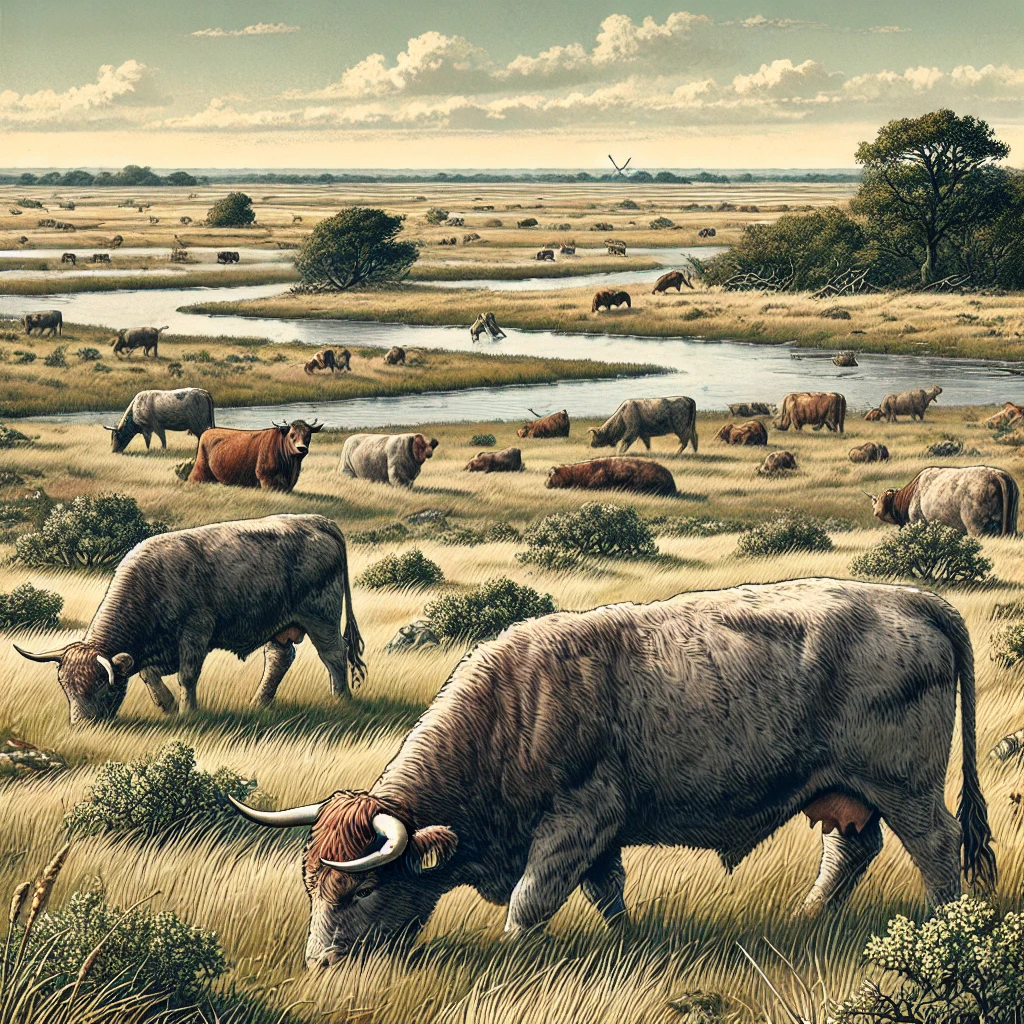
\includegraphics[width=0.8\textwidth,height=\textheight]{figuren/heck_ai.png}

}

\caption{Afbeelding gegenereerd met ChatGPT4-o}

\end{figure}%

\subsection{Geboorte en sterfte}\label{geboorte-en-sterfte}

In het vorige onderdeel hebben we dichtheidsafhankelijkheid ingebouwd
zodat de populatie langzamer gaat groeien bij grote dichtheden:

\[
\frac{\mathrm{d}N}{\mathrm{d}t} = rN\left(1-\frac{N}{K}\right)
\]

De parameter \(r\) in deze vergelijking staat bekend als de
\textbf{intrinsieke groeisnelheid} (\emph{intrinsic growth rate}) van de
populatie. Als \(r\) positief is, is er groei (ook als \(r=0.1\)!). Als
\(r\) negatief is, is de groei negatief. Maar biologisch gezien is
``negatieve groei'' natuurlijk een beetje vreemd. Bedoelen we niet
eigenlijk dat de hoeveelheid sterfte (hierna: \emph{death}) hoger is dan
geboorte (hierna: \emph{birth})? Een gebrek aan voedsel kan bijvoorbeeld
een verhoogde death rate opleveren, terwijl birth rate gelijk blijft.
Het zou ook zo kunnen zijn dat individuen met minder voedsel minder
reproduceren (dus een verlaagde birth rate krijgen). Om deze verbale
begrippen in onze ODE te verwerken, moeten we afstappen van de parameter
\(r\), en deze uitsplitsen in birth (\(b\)) en death (\(d\)).
Bijvoorbeeld, neem ons model van exponentiële groei:

\[
    \frac{\mathrm{d}N}{\mathrm{d}t} = rN 
\] Nogmaals: in dit model is er exponentiele groei wanneer \(r>0\), en
exponentiele afname wanneer \(r<0\). Als we r vervangen door het
verschil in birth (\(b\)) en death (\(d\)), dan krijgen we:

\begin{equation}\phantomsection\label{eq-rbd}{
    \frac{\mathrm{d}N}{\mathrm{d}t} = ( {\color{blue}b} - {\color{red}d} )N
}\end{equation}

\begin{tcolorbox}[enhanced jigsaw, colframe=quarto-callout-caution-color-frame, title=\textcolor{quarto-callout-caution-color}{\faFire}\hspace{0.5em}{Let op! Equation~\ref{eq-rbd} geeft ook gewoon exponentiele groei (of
afname)!}, colbacktitle=quarto-callout-caution-color!10!white, titlerule=0mm, rightrule=.15mm, colback=white, toptitle=1mm, toprule=.15mm, arc=.35mm, bottomtitle=1mm, opacitybacktitle=0.6, bottomrule=.15mm, leftrule=.75mm, left=2mm, coltitle=black, breakable, opacityback=0]

Hoewel we twee nieuwe parameters hebben geintroduceerd, is er weinig
veranderd aan ons model. Net als dat \(r>0\) en \(r<0\) respectievelijk
leidde tot groei en afname, is er bij \(b>d\) en \(b<d\) ook sprake van
exponentiële groei of afname:

\begin{center}
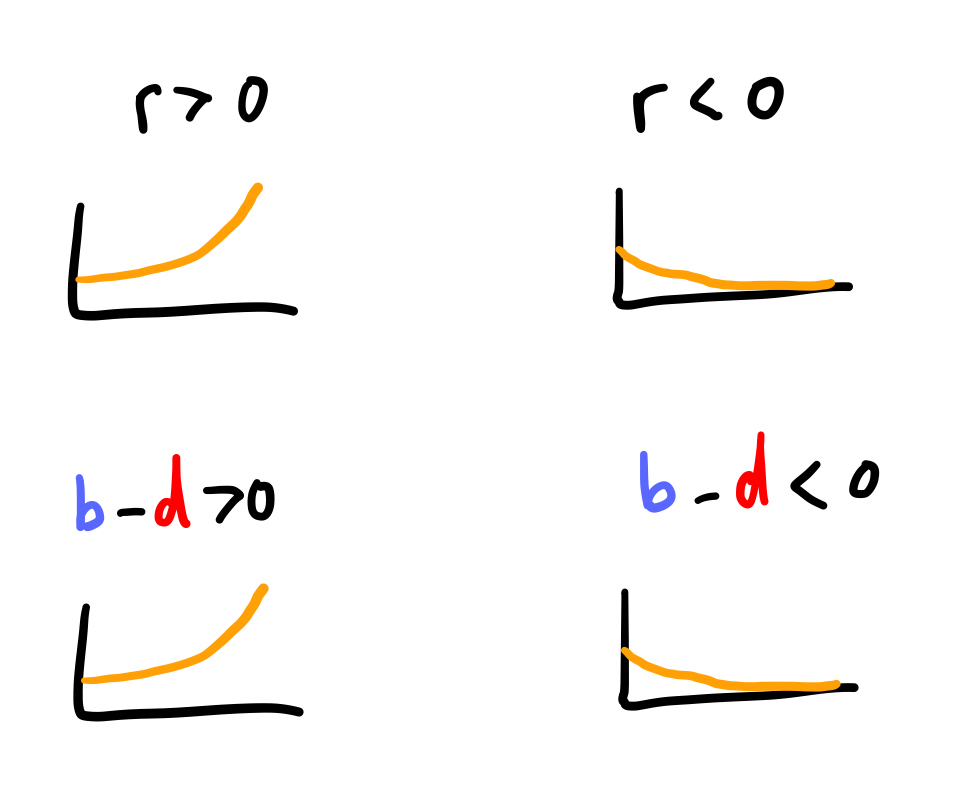
\includegraphics[width=0.5\textwidth,height=\textheight]{figuren/exponential_with_bd_vs_r.png}
\end{center}

\end{tcolorbox}

\subsection{Dichtheidsafhankelijke
geboorte}\label{dichtheidsafhankelijke-geboorte}

Hoewel onze nieuwe vergelijking voor groei nog niet heel anders is,
kunnen we met deze aanpassing wel na gaan denken over \emph{birth} en
\emph{death} processen. Stel je voor dat we experimenteel hebben bepaald
dat een soort dichtheidsafhankelijke geboorte heeft (\emph{density
dependent birth}), zie bijvoorbeeld Figure~\ref{fig-ddbpears}.

\begin{figure}

\centering{

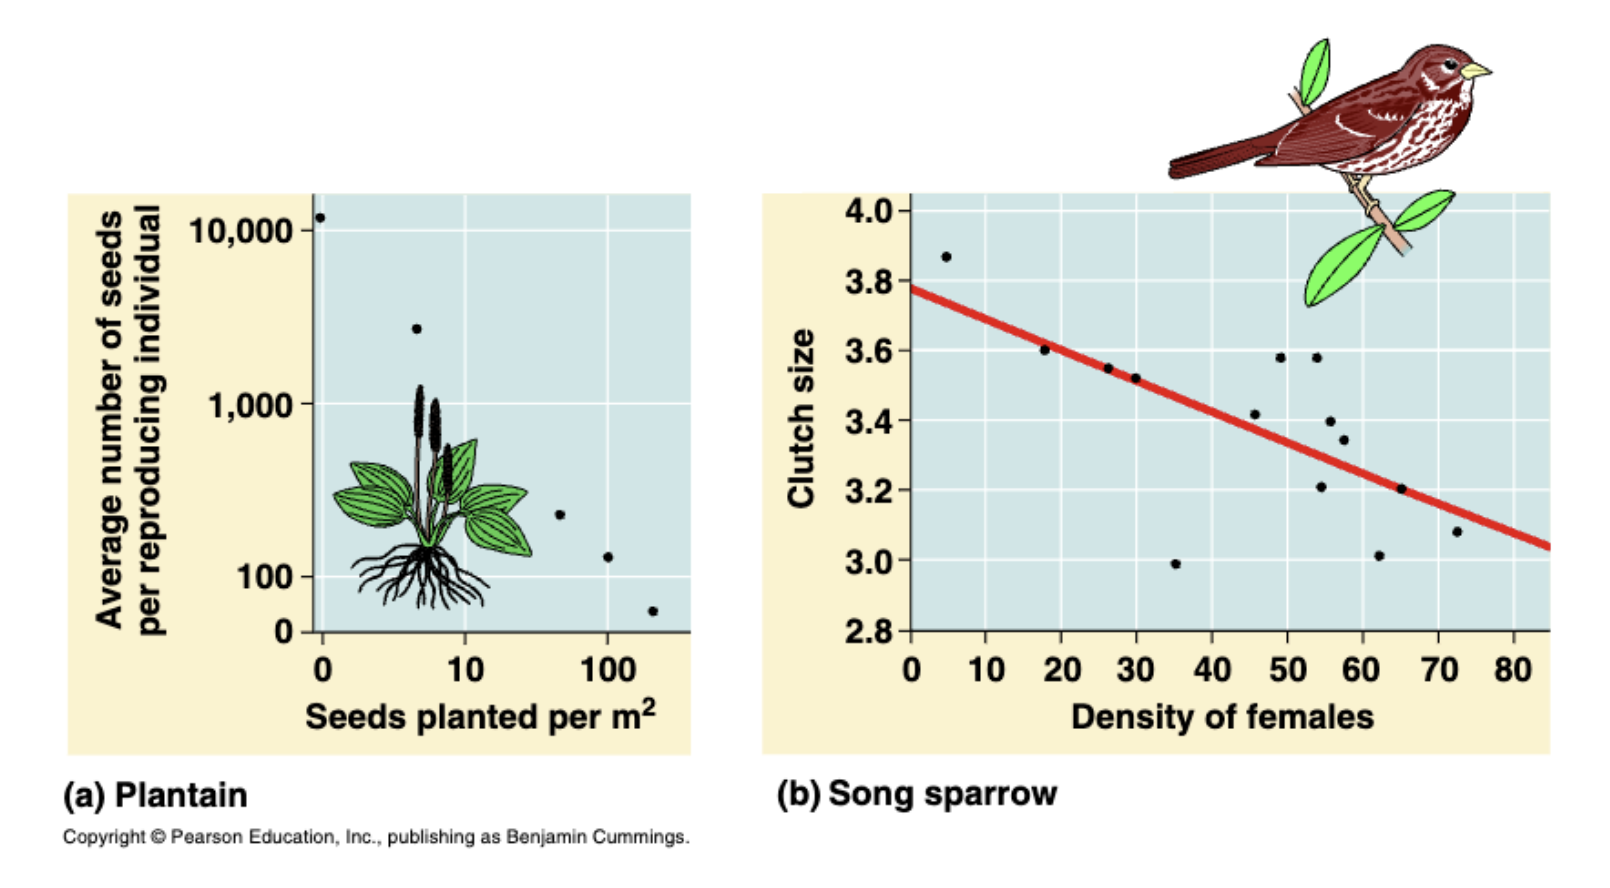
\includegraphics{figuren/ddb_pears.png}

}

\caption{\label{fig-ddbpears}Reproductiesucces neemt vaak af met
dichtheid (© 2014 Pearson Education Inc.)}

\end{figure}%

Waar we deze afname eerder in het gehele groei-process hadden verwerkt
door aan te nemen dat \(r\) kleiner werd, gaan we nu een nieuw model
bekijken waar alleen de birth verandert bij grotere dichtheden. Hiervoor
is het handig om eerst de birth en death termen op te splitsen:

\begin{align}
    \frac{\mathrm{d}N}{\mathrm{d}t} &= (\color{blue}b\color{black}-\color{red}d\color{black})N\\
    \frac{\mathrm{d}N}{\mathrm{d}t} &= \color{blue}b\color{black}N - \color{red}d\color{black}N
\end{align}

Nu kunnen we ervoor kiezen om voor de geboorteterm met een
\textbf{functionele response} aan te passen:

\begin{align}
    \color{blue}b\color{black} & \rightarrow \color{blue}b\color{black} \cdot f(N)
\end{align}

Bijvoorbeeld dezelfde functionele response die we eerder hebben
gebruikt:

\begin{align}
    \color{blue}b\color{black} & \rightarrow \color{blue}b\color{black}\left(1-\frac{N}{K}\right) 
\end{align}

Dat wil zeggen, de constante parameter \(b\) wordt vervangen door een
term die afneemt met \(N\). De parameter \(b\) staat nu niet meer voor
de birth rate, maar voor de \emph{maximale birth rate} die alleen
bereikt wordt bij kleine populatiegroottes. Als we dit in de gehele ODE
invullen, krijgen we nu:

\begin{align}
    \frac{\mathrm{d}N}{\mathrm{d}t} &= \color{blue}b\color{black}\left(1-\frac{N}{K})N - \color{red}d\color{black}N
\end{align}

\begin{exercise}[Andere functionele
responses]\protect\hypertarget{exr-functioneleresponses}{}\label{exr-functioneleresponses}

Hierboven gebruiken we de functionele response \(f(N)=1-\frac{N}{K}\) om
geboorte af te laten nemen. Leg uit waarom de volgende functionele
responses wel/niet een vergelijkbaar effect zullen hebben:

\begin{enumerate}
\def\labelenumi{\alph{enumi}.}
\tightlist
\item
  \(f(N)=\frac{N}{K} + 1\)
\item
  \(f(N)= 1 - cN\)
\item
  \(f(N)= 1 - cN^2\)
\end{enumerate}

\end{exercise}

\subsection{Het faseportret}\label{het-faseportret}

Zoals je in het vorige hoofdstuk geleerd hebt, kunnen we ODEs eenvoudig
analyseren door ons af te vragen: wanneer is er geen groei meer? Wanneer
is \(\mathchoice{\frac{\mathrm{d}N}
{\mathrm{d}t}}{\mathrm{d}N/\mathrm{d}t}
{\mathrm{d}N/\mathrm{d}t}
{\mathrm{d}N/\mathrm{d}t}\) gelijk aan \(0\)? Deze relatief eenvoudige
berekening word weergegeven in de linkerzijde van
Figure~\ref{fig-faseportret}. De rechterzijde geeft visueel weer wat
deze berekening nou eigenlijk heeft bepaald, door de groeisnelheid (dus:
de ODE) als functie van de dichtheid van de populatie te schetsen. Als
we de ODE uitvermenigvuldigen zien we een negatieve tweede-orde term
(\(-bN^2/k\)) en twee eerste-orde termen (\(bN\) en \(dN\) zijn niet
gekwadrateerd). Dit vormt een bergparabool\footnote{Als je functies
  schetsen lastig vindt, kijk dan nog even naar
  \hyperref[section-schetsen]{hoofdstuk 10}. Je kan het ook altijd even
  controleren met de website \href{https://www.desmos.com}{Desmos.com}},
een functie die op twee punten gelijk is aan \(0\). Op deze punten is de
populatie in evenwicht: deze kan niet groeien of krimpen.

\begin{figure}

\centering{

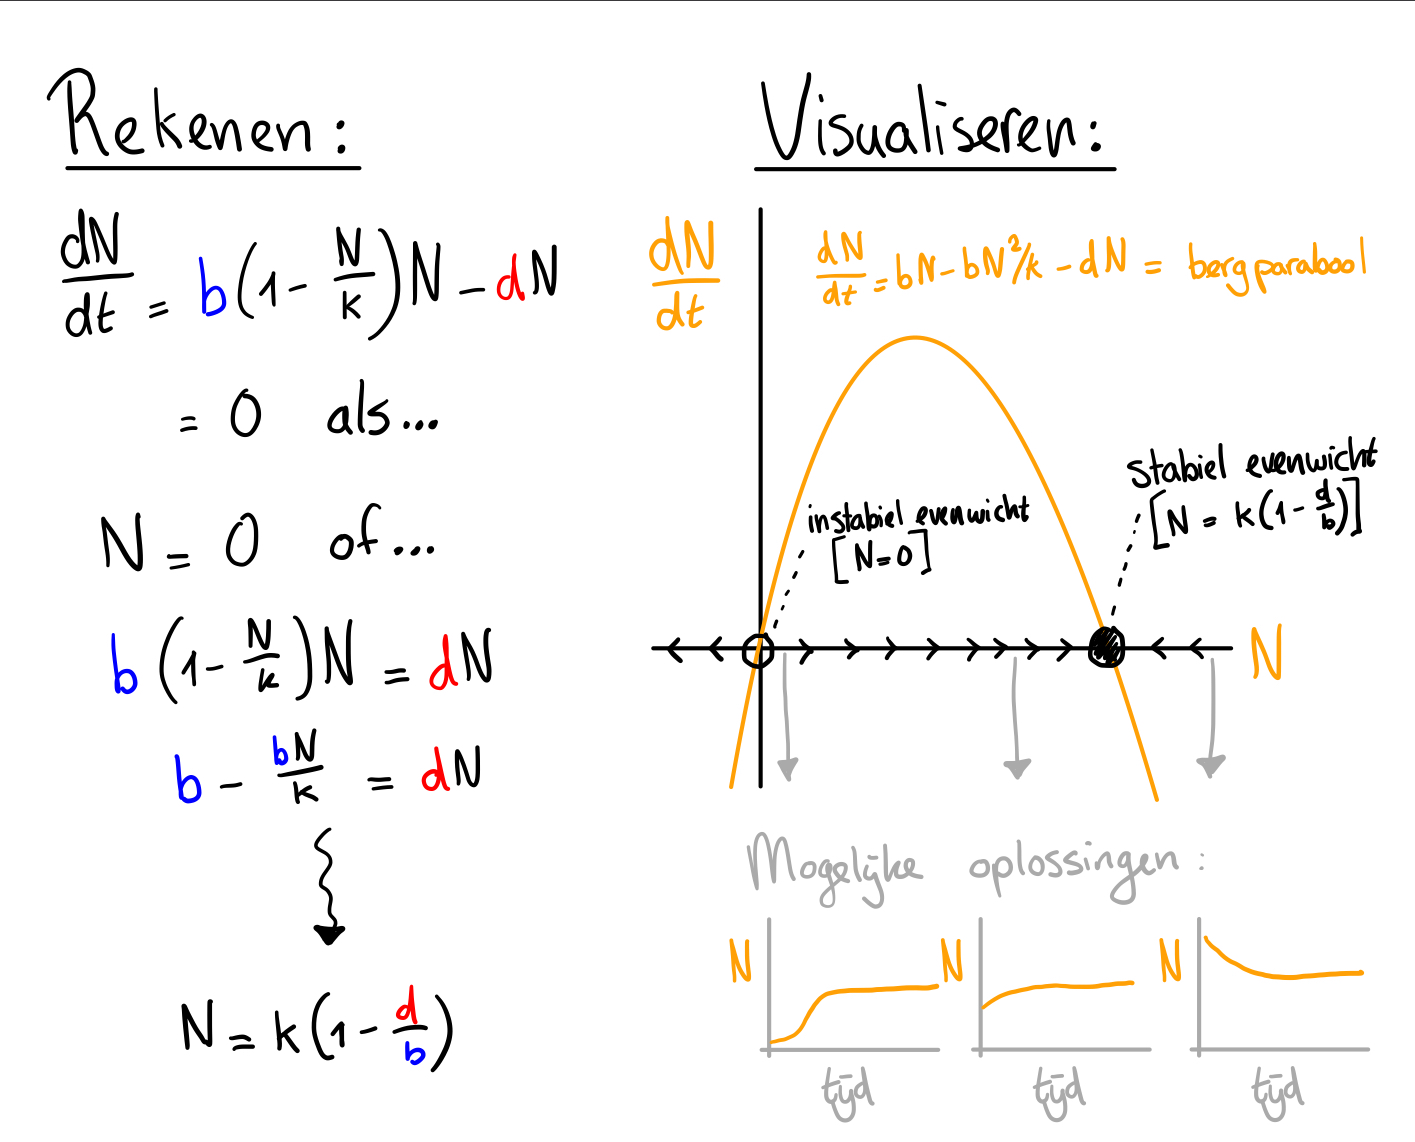
\includegraphics[width=0.8\textwidth,height=\textheight]{figuren/faseportret_logistische_groei.png}

}

\caption{\label{fig-faseportret}Rekenen aan evenwichten, of deze
visualiseren in een faseportret}

\end{figure}%

Er is nog iets wat je heel snel aan een faseportret af kan lezen. We
weten dat er groei is als \(\mathchoice{\frac{\mathrm{d}N}
{\mathrm{d}t}}{\mathrm{d}N/\mathrm{d}t}
{\mathrm{d}N/\mathrm{d}t}
{\mathrm{d}N/\mathrm{d}t}\) groter is dan \(0\) en dat de populatie
afneemt als \(\mathchoice{\frac{\mathrm{d}N}
{\mathrm{d}t}}{\mathrm{d}N/\mathrm{d}t}
{\mathrm{d}N/\mathrm{d}t}
{\mathrm{d}N/\mathrm{d}t}\) kleiner is dan \(0\) (en zoals gezegd: dat
er een evenwicht is als \(\mathchoice{\frac{\mathrm{d}N}
{\mathrm{d}t}}{\mathrm{d}N/\mathrm{d}t}
{\mathrm{d}N/\mathrm{d}t}
{\mathrm{d}N/\mathrm{d}t}\) gelijk is aan \(0\)). In het figuur staan
deze punten aangegeven op de x-as. Pijltjes naar rechts geven aan dat er
groei is (pijltje wijst naar ``meer N''), pijltjes naar links geven aan
dat er afname is, en cirkels geven aan dat er een evenwicht is. Als de
pijltjes naar dit evenwicht toewijzen, dan zal het systeem daar op ten
duur naartoe gaan. Zo'n \textbf{stabiel evenwicht} wordt ook wel een
\textbf{attractor} genoemd, en wordt vaak aangegeven met een ingevulde
cirkel. Het evenwicht bij \(N=0\) heeft alleen pijltjes die ervan
wegwijzen, en is dus een \textbf{instabiel evenwicht} (en is geen
attractor). Deze worden vaak aangegeven met een open cirkel. Dankzij
deze visualisatie is het relatief eenvoudig om te bedenken hoe het
systeem zich over de tijd zal ontwikkelen. Voor specifieke
begin-waarden, kunnen we dus \emph{specifieke oplossingen} schetsen!

\subsection{Dichtheidsafhankelijke
sterfte}\label{dichtheidsafhankelijke-sterfte}

Op een vergelijkbare manier als hierboven, zouden we ook een populatie
kunnen modelleren die dichtheidsafhankelijke sterfte (\emph{density
dependent death}) ondergaat:

\begin{align}
    \color{red}d\color{black} & \rightarrow \color{red}d\color{black}(1+\frac{N}{K}) \\
    \frac{\mathrm{d}N}{\mathrm{d}t} &= \color{blue}b\color{black}N - \color{red}d\color{black}(1+\frac{N}{K})N
\end{align}

Let op dat we hier de sterfte laten \emph{toenemen} met de dichtheid (er
staat een \(+\) in plaats van een \(-\)).

\begin{exercise}[Rekenen aan dichtheidsafhankelijke
sterfte]\protect\hypertarget{exr-dddportrait}{}\label{exr-dddportrait}

Hierboven hebben we een ODE opgesteld voor dichtheidsafhankelijke
sterfte, namelijk: \[
\frac{\mathrm{d}N}{\mathrm{d}t} = \color{blue}b\color{black}N - \color{red}d\color{black} \left( 1+\frac{N}{K}\right)N
\] Bekijk nog eens Figure~\ref{fig-faseportret}.

\begin{enumerate}
\def\labelenumi{\alph{enumi}.}
\tightlist
\item
  Bereken waar de evenwichten liggen met de dichtheidsafhankelijke
  sterfte
\item
  Schets het faseportret en geef aan waar eventuele evenwichten liggen.
\end{enumerate}

\end{exercise}

\subsection{Andere dichtheidseffecten}\label{andere-dichtheidseffecten}

In de natuur zal het vaak zo zijn dat zowel geboorte als sterfte door de
populatiegrootte worden beinvloed, dus moeten we ook beide in ons model
opnemen. Dan krijgen we:

\begin{align}
    \frac{\mathrm{d}N}{\mathrm{d}t} &= \color{blue}b\color{black}(1-\frac{N}{K_b})N - \color{red}d\color{black}(1+\frac{N}{K_d})N\\
\end{align}

Hier schaalt \(K_b\) de dichtheidsafhankelijke geboorte, en \(K_d\) de
dichtheidsafhankelijke sterfte. In het werkcollege zullen jullie zien
dat dit simpele model inzicht kan geven in belangrijke
beleidsbeslissingen met betrekking tot dierenwelzijn.

Er zijn vele andere mogelijke dichtheidseffecten mogelijk (teveel om te
benoemen). Als we het over ecosystemen hebben, zullen er ook effecten
zijn die afhangen van de dichtheid van een \emph{andere} soort. We
kunnen ons bijvoorbeeld voorstellen dat de konijnen (\(N\)) door vossen
(\(V\)) worden opgegeten. Hoe meer konijnen en vossen, hoe
waarschijnlijker het wordt dat konijnen worden weggegeten: dus dit is
ook een dichtheidseffect:

\begin{align}
    \frac{\mathrm{d}N}{\mathrm{d}t} &= \color{blue}b\color{black}(1-\frac{N}{K_b})N - \color{red}d\color{black}(1+\frac{N}{K_d})N - cNV\\
\end{align}

Deze vergelijking begint er aardig ingewikkeld uit te zien, maar doordat
we het stapje voor stapje hebben opgebouwd, zie je wellicht goed in wat
elke term betekent. In de laatste (nieuwe term), staat \(c\) voor de
predatiesnelheid is en \(V\) de hoeveelheid vossen. Maar vossen zouden
zelf dan toch ook van populatiegrootte moeten veranderen? In
\textbf{?@sec-meerdere} ga je zien hoe we ons model kunnen uitbreiden om
zowel konijnen (prooi) als vossen (predator) te kunnen beschrijven.

\subsection{Opgaven}\label{opgaven}

\begin{exercise}[Bacteriën in het
bloed]\protect\hypertarget{exr-bacterienbloed}{}\label{exr-bacterienbloed}

\begin{figure}[H]

{\centering 
\includegraphics[width=0.8\textwidth,height=\textheight]{figuren/tandenpoetsen.png}

}

\caption{Afbeelding gegenereerd met ChatGPT4-o}

\end{figure}%

Elke keer dat je je tanden poetst, komt er een kleine hoeveelheid
bacteriën in je bloed. Omdat bloed een erg voedselrijke omgeving is voor
bacteriën, zouden ze hier onmiddelijk exponentieel kunnen groeien.
Gelukkig hebben we neutrofielen in ons bloed die de bacteriën snel
opruimen. Hier zouden we een simpel ODE model voor opstellen:

\[\mathchoice{\frac{\mathrm{d}B}
{\mathrm{d}t}}{\mathrm{d}B/\mathrm{d}t}
{\mathrm{d}B/\mathrm{d}t}
{\mathrm{d}B/\mathrm{d}t}=rB-kNB \]

Hier is B de hoeveelheid bacterien in je bloed is, N de hoeveelheid
neutrofielen in je bloed, \(r\) de groeisnelheid van de bacteriën (per
uur), en k de snelheid waarmee neutrofielen bacteriën opruimen.

\begin{enumerate}
\def\labelenumi{\alph{enumi}.}
\tightlist
\item
  Leg uit waar je denkt dat iedere term in de ODE voor staat (\(rB\) en
  \(=kNB\)), en welke eenheden deze termen hebben.
\item
  Wat zijn de eenheden voor \(r\) en \(k\)?
\end{enumerate}

Als er geen bacteriën zijn (\(B=0\)) is er geen groei. Dit wordt een
triviaal (irrelevant) evenwicht genoemd, omdat we voor dit inzicht het
hele model niet hadden hoeven maken.

\begin{enumerate}
\def\labelenumi{\alph{enumi}.}
\setcounter{enumi}{2}
\item
  Neem aan dat er een constante hoeveelheid neutrofielen in je bloed
  zijn (\(N\) is constant). Is er een niet-triviaal evenwicht van
  bacteriën?
\item
  Chemotherapie kan een groot effect hebben op het aantal neutrofielen
  in het bloed, waardoor de tweede term steeds kleiner wordt. Schets de
  termen \(rB\) en \(kNB\) als een functie van \(N\) (dat wil zeggen,
  met \(N\) op de x-as, en deze termen op de y-as.
\item
  Bepaal hoeveel neutrofielen je minimaal nodig hebt om de groei van de
  bacteriën te stoppen.
\item
  De \(kNB\) term heet een \emph{mass-action} term omdat de snelheid
  direct proportioneel is aan de dichtheden van \(N\) en \(B\). Wat
  moeten we doen als we willen weten hoeveel bacteriën er ``per
  neutrofiel'' opgeruimd worden?
\item
  Hoeveel bacteriën worden er per neutrofiel opgeruimd als er 0
  bacteriën zijn? En als er oneindig bacteriën zijn? Is dit een
  redelijke aanname?
\end{enumerate}

Bekijk devolgende uitbreiding van ons model
\[\mathchoice{\frac{\mathrm{d}B}
{\mathrm{d}t}}{\mathrm{d}B/\mathrm{d}t}
{\mathrm{d}B/\mathrm{d}t}
{\mathrm{d}B/\mathrm{d}t}=rB-\frac{kNB}{h+B}  \] De vernieuwde (tweede)
term ziet er misschien wat ingewikkeld uit. Om te begrijpen wat er
gebeurt is het wederom handig om even na te gaan wat er gebeurt met 0 of
heel veel bacterien. Als er 0 bacterien zijn is deze term 0, omdat boven
de breuk een \(B\) staat.

\begin{enumerate}
\def\labelenumi{\alph{enumi}.}
\setcounter{enumi}{7}
\item
  Als \(B\) heel groot is, hoe belangrijk is \(h\) dan nog in deze
  vergelijking?
\item
  Als er dus heel veel bacterien zijn, hoeveel bacterien kunnen er dan
  per neutrofiel opgeruimd worden in dit nieuwe model?
\item
  Bepaal opnieuw hoeveel neutrofielen je minimaal nodig hebt om de groei
  van bacteriën te stoppen.
\end{enumerate}

\end{exercise}

\begin{exercise}[Heckrunderen]\protect\hypertarget{exr-heck}{}\label{exr-heck}

Heckrunderen zijn in de Oostvaardersplassen geintroduceerd als
``semi-natuurlijke'' grazers. Ze voorkomen dat het hele gebied begroeid
raakt met bomen en struikgewas, wat belangrijk is voor het broeden van
vogels in dit gebied. In 1983 zijn een kleine populatie heckrunderen
vrijgelaten, en de populatie is na 20 jaar gestabiliseerd op 300-400
runderen.

\begin{figure}

\centering{

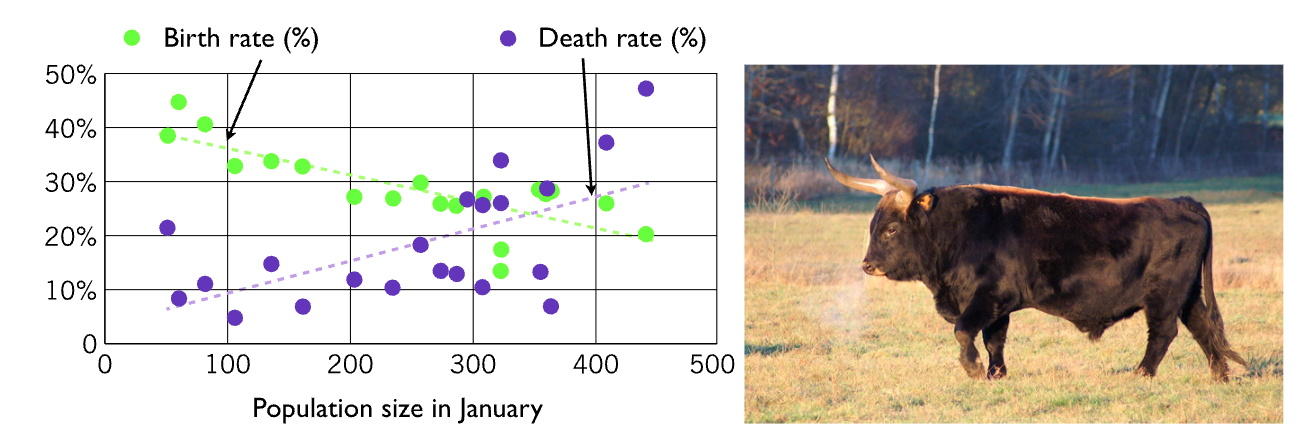
\includegraphics{figuren/heck.png}

}

\caption{\label{fig-heck}Heckrunderen op de Oostvaardersplassen}

\end{figure}%

Omdat er veel dieren van de honger doodgaan, zijn er veel debatten
geweest over dierenwelzijn. Een mogelijke oplossen is het afschieten van
dieren. Dit zou hun populatiegrootte kunnen verkleinen en daardoor de
overgebleven individuen een prettiger leven geven.

\begin{enumerate}
\def\labelenumi{\alph{enumi}.}
\tightlist
\item
  Bekijk bovenstaande metingen van de geboorte- en sterfte van
  heckrunderen. Hoeveel heckrunderen zou je op basis van deze data
  verwachten in evenwicht?
\end{enumerate}

De data laat zien dat zowel geboorte als sterfte dichtheidsafhankelijk
zijn. In het hoofdstuk hebben we hier al een model voor besproken: \[
      \frac{\mathrm{d}N}{\mathrm{d}t} = \color{blue}b\color{black}\left(1-\frac{N}{K_b}\right)N - \color{red}d\color{black}\left(1+\frac{N}{K_d}\right)N
  \]

Uit het figuur kunnen we zien dat geboorte per rund hoogstens 0.4 per
jaar is, en dat deze bij 400 runderen gehalveerd is.

\begin{enumerate}
\def\labelenumi{\alph{enumi}.}
\setcounter{enumi}{1}
\tightlist
\item
  Wat zijn dan de parameters \(b\) en \(K_b\)?
\item
  In de figuur zien we ook dat sterfte minimaal 0.03 is, en dat deze
  0.33 is bij een populatiegrootte van 500. Wat zijn dan de parameters
  \(d\) en \(K_d\)?
\item
  Vul de parameterwaarden die hebt gevonden in, en bepaal bij welke
  populatiegrootte er een evenwicht is.
\item
  Hoeveel dieren gaan er in dit evenwicht per jaar dood?
\end{enumerate}

Om het afschieten van runderen in dit model te betrekken, kunnen we een
extra term aan de ODE toevoegen: \[
      \frac{\mathrm{d}N}{\mathrm{d}t} = \color{blue}b\color{black}(1-\frac{N}{K_b})N - \color{red}d\color{black}(1+\frac{N}{K_b})N - kN
  \] Waarbij \(k\) de fractie runderen is die we afschieten. Bekijk
hetvolgende R-script:

\begin{verbatim}
::: {.cell}

```{.r .cell-code  code-fold="false"}
# Stap 1: Een functie die verandering uitrekent
verandering <- function (N){
  delta <- b*(1-(N/Kb))*N - d*(1+(N/Kd))*N - k*N
  return(delta)
}

# Stap 2: stel begin-aantal / parameters in
N <- 10
b <- 0.4    
d <- 0.03
Kb <- 800
Kd <- 50
k <- 0.0

# Stap 3, definieer tijdstappen en maak een dataframe aan
delta_t <- 0.1 # grootte van de tijdstap
tijdstapjes <- seq(0,50,by=delta_t)
tijdserie <- data.frame(t=tijdstapjes,runderen=N,sterfte=NA)

for (t in 1:length(tijdstapjes)-1) {
  if(t>300) k <- 0.05
  sterfte <- N*d*(1+N/Kd) + k*N
  N <- N + delta_t*verandering(N)
  tijdserie[t+1,] <- c(t=t*delta_t, runderen=N, sterfte=sterfte)
}

# Plot het totaal aantal heckrunderen door de tijd
plot(tijdserie$t, tijdserie$runderen, xlab="Tijd in jaren", ylab="Aantal heckrunderen", type="l", col="brown", lwd=2)
# Plot het aantal stervende heckrunderen
lines(tijdserie$t, tijdserie$sterfte, col="red", lty=2)
# Voeg legenda toe
legend(40, 270, legend=c("Totaal", "Sterfte"), col=c("brown", "red"), lty=1:2)
```
:::
\end{verbatim}

\begin{enumerate}
\def\labelenumi{\alph{enumi}.}
\setcounter{enumi}{5}
\tightlist
\item
  Na hoeveel jaar wordt er begonnen met schieten? Welk percentage van de
  heckrunderen wordt afgeschoten?
\end{enumerate}

Met \texttt{tijdserie\$runderen/tijdserie\$sterfte} kunnen we de
sterfte-kolom delen door de kolom met het totaal aantal runderen om uit
te rekenen welk percentage van de populatie op elk tijdstap sterft (let
op: sterfte is inclusief afschieten!). Deze zouden we ook kunnen
toevoegen aan ons dataframe, en apart kunnen plotten:

\begin{verbatim}
::: {.cell}

```{.r .cell-code  code-fold="false"}
tijdserie$percentage_sterfte = tijdserie$sterfte/tijdserie$runderen
plot(tijdserie$t, tijdserie$percentage_sterfte, type="l")
```
:::
\end{verbatim}

\begin{enumerate}
\def\labelenumi{\alph{enumi}.}
\setcounter{enumi}{6}
\item
  Bekijk het nieuwe dataframe met \texttt{View(tijdserie)}, en vergelijk
  het percentage sterfte in jaar 30 en 50. Wat valt je op?
\item
  Met het percentage stervende dieren kunnen we inschatten hoe lang de
  dieren gemiddeld leven. Als 10\% van de dieren jaarlijks overlijdt,
  dan leeft een dier gemiddeld 10 jaar. Als je dit combineert met je
  antwoord op de vorige vraag, zou je het afschieten van dieren dan
  aanmoedigen of afraden?
\item
  Als je de verwachte levensduur zo min mogelijk wil beinvloeden, wat
  voor beleid zou je dan nog meer kunnen bedenken?
\end{enumerate}

\end{exercise}

\subsection{Terminologie}\label{terminologie}

\begin{longtable}[]{@{}
  >{\raggedright\arraybackslash}p{(\columnwidth - 4\tabcolsep) * \real{0.2500}}
  >{\raggedright\arraybackslash}p{(\columnwidth - 4\tabcolsep) * \real{0.2778}}
  >{\raggedright\arraybackslash}p{(\columnwidth - 4\tabcolsep) * \real{0.4722}}@{}}
\toprule\noalign{}
\begin{minipage}[b]{\linewidth}\raggedright
Nederlands
\end{minipage} & \begin{minipage}[b]{\linewidth}\raggedright
Engels
\end{minipage} & \begin{minipage}[b]{\linewidth}\raggedright
Beschrijving
\end{minipage} \\
\midrule\noalign{}
\endhead
\bottomrule\noalign{}
\endlastfoot
Intrinsieke groeisnelheid & Intrinsic growth rate & De snelheid waarmee
een populatie groeit, weergegeven als \(r\). Hierbij is niet
gedefiniëerd wat de precieze geboorte- en sterftesnelheden zijn. \\
Dichtheidsafhankelijk & Density dependent & Wanneer een process sneller
of langzamer gaat als de dichtheid (of een andere soort variabele)
verandert \\
Faseportret & Phase portrait & Een visuele manier om van een ODE weer te
geven waar de eventuele evenwichten liggen, en of deze instabiel/stabiel
zijn \\
Evenwicht & Steady state & Een conditie waarbij een systeem niet
verandert. Bijvoorbeeld, een populatiegrootte waarbij er geen
groei/afname is. \\
Stabiel evenwicht & Stable steady state & Een evenwicht waar het systeem
naartoe beweegt, bijvoorbeeld wanneer de groeisnelheid toeneemt bij
afname, en afneemt bij toename. \\
Instabiel evenwicht & Unstable steady state & Een evenwicht waar het
systeem van weg beweegt, bijvoorbeeld wanneer de groeisnelheid toeneemt
bij toename, en afneemt bij afname. Dit zijn dus weliswaar evenwichten,
maar elk mogelijke verstoring zal het systeem ervandaan bewegen! \\
Attractor & Attractor & Waar het systeem naartoe gaat als je lang genoeg
wacht. Vaak is dit een stabiel evenwicht, maar er dit is niet altijd het
geval! \\
Massawerking & Mass action & Mass action (het Nederlandse begrip is
ongebruikelijk) is een aanname dat interacties tussen
individuen/moleculen direct proportioneel is aan de
dichtheden/concentraties. \\
\end{longtable}




\end{document}
